\documentclass{beamer}
\usepackage[utf8]{inputenc}
\usepackage[T1]{fontenc}
\usepackage{amsmath}
\usepackage{physics}
\usepackage{graphicx}
\usepackage{float}
\usepackage{siunitx}
\usepackage{amsfonts}
\usepackage{amssymb}
\usepackage{amsthm}
%\usepackage[export]{adjustbox}
\usepackage{subcaption}
\usepackage{bm}
\usepackage{cancel}
\usepackage{comment}
\usepackage{enumerate}
\usepackage{centernot}
\usepackage{mathtools}
\usepackage{mathrsfs}

\newcommand{\tonde}[1]{\left( {#1} \right)}
\newcommand{\quadre}[1]{\left[ {#1} \right]}
\newcommand{\graffe}[1]{\left\{ {#1} \right\}}
\theoremstyle{remark}
\newtheorem*{nota}{Nota}

\usepackage{animate}
\newcommand{\nologo}{\setbeamertemplate{logo}{}} % command to set the logo to nothing

\usepackage{hyperref}
\hypersetup{
    colorlinks=true,
    linkcolor=blue,
    filecolor=magenta,      
    urlcolor=cyan,
    citecolor=blue,%mancava questo! Senza mette il verde di default. O gray
    pdftitle={Tesi Marco Giunta},
    bookmarks=true,
    pdfpagemode=FullScreen,
}
\urlstyle{same}

\let\temp\phi%questi comandi scambiano phi e varphi
\let\phi\varphi
\let\varphi\temp

\renewcommand{\L}{\mathcal{L}}
\newcommand{\N}{\mathcal{N}}
\usepackage{bbm} % per fare l'1 mathbb


\usepackage{csquotes}%lo consiglia lui
\usepackage[
    backend=biber,
    %style=alphabetic%authortitle,%se no numeric. Questo è per cambiare cosa spunti alla fine
    %bibencoding=ascii,
    %citestyle=alphabetic%authoryear%authortitle,%se no numeric. Questo cambia cosa si veda nel testo %se no alphabetic/authoryear in entrambi
    sorting=nyt %sort by name, year, title
]{biblatex}

\addbibresource{miabibliografia.bib} %Imports bibliography file
%------------------------------------------------------------
%This block of code defines the information to appear in the
%Title page
\title[astroABC]{astroABC: An Approximate Bayesian Computation
Sequential Monte Carlo sampler for cosmological
parameter estimation}
\subtitle{\textit{paper by E. Jennings \& M. Madigan}}
\author{Marco Giunta}
\date[21/06/22]{21 June 2022}

\logo{\includegraphics[height=1.3cm]{Logo_Università_Padova.png}}
%End of title page configuration block
%------------------------------------------------------------

\usepackage{utopia} %font utopia imported

\usetheme{Madrid}
\usecolortheme{default}
\setbeamertemplate{sections/subsections in toc}[default]
\setbeamertemplate{enumerate items}[default] % per togliere le palle da enumerate e lasciare solo i numeri.
% nello stile di default enumerate ha solo i numeri, che vengono sovrascritti dalle palle numerate di Madrid

%------------------------------------------------------------
%The next block of commands puts the table of contents at the 
%beginning of each section and highlights the current section:
\AtBeginSection[]
{
  \begin{frame}
    \frametitle{Table of Contents}
    \tableofcontents[currentsection]
  \end{frame}
}
%------------------------------------------------------------


\begin{document}

%The next statement creates the title page.
\frame{\titlepage}


\begin{frame}{Introduction}
From the paper abstract: 

\textit{
``Given the complexity of modern cosmological parameter inference where
we are faced with non-Gaussian data and noise, correlated systematics and
multi-probe correlated data sets, the Approximate Bayesian Computation
(ABC) method is a promising alternative to traditional Markov Chain Monte
Carlo approaches in the case where the Likelihood is intractable or unknown.
The ABC method is called “Likelihood free” as it avoids explicit evaluation
of the Likelihood by using a forward model simulation of the data which can
include systematics. We introduce astroABC, an open source ABC Sequential Monte Carlo (SMC) sampler for parameter estimation. [\dots]''}
\end{frame}



%---------------------------------------------------------
%This block of code is for the table of contents after
%the title page
\begin{frame}
\frametitle{Table of Contents}
\tableofcontents
\end{frame}
%---------------------------------------------------------



\section{Why Likelihood-free methods?}
\begin{frame}{Bayesian parameter inference pipeline}
Any Bayesian parameter inference problem is made of three ingredients:
\begin{equation*}
    \text{Prior} \ \pi(\theta) \to \text{Likelihood} \ \L(D|\theta) \to \text{Posterior} \ P(\theta|D)
\end{equation*}
Defining each of these terms has its own challenges:\pause
\begin{itemize}[<+->]
    \item How do we effectively incorporate prior knowledge (previous surveys, physical constraints) in the problem, or lack thereof (uninformative priors)?
    \item How do we accurately model the problem (theoretical \& error contributions)?
    \item How do we actually implement Bayes' theorem (MCMC, etc.)?
\end{itemize}
\pause[\thebeamerpauses]
From now on we assume fixing the prior is not an issue \& focus on the likelihood
\end{frame}

\begin{frame}{Assembling $\L(\theta|D)$}
In order to construct a likelihood appropriate to our problem we must have theoretical results linking variables and a model for the errors involved
\pause
\begin{itemize}[<+->]
    \item Trivial example: 1D linear regression with gaussian errors of fixed variance on $y$, no errors on $x$
    \begin{equation*}
        \hat{y}_i = ax_i + b + \varepsilon_i, \ \varepsilon_i \sim N(0, \sigma^2) \implies \L(\va{y}|a,b)\propto \prod_{i=1}^N\exp(-\frac{y_i - ax_i - b}{2\sigma^2})
    \end{equation*}
    \item Cosmological example: SN Ia datasets
    \begin{equation*}
    \begin{cases}
        \mu_i = m_{Bi}-M_i+\alpha x_{1i}+\beta c_i\\
        M_i\sim \N(M_0, (\sigma_\mu^{\text{int}})^2)\\
        \hat{z}_i \sim \N(z_i,\sigma_z^2)\\
        \vdots
    \end{cases}
    \implies \L(D|\va{\theta}) = \dots \ (\text{BHM})
    \end{equation*}
\end{itemize}
\end{frame}


\begin{frame}{ABC-friendly Likelihoods}
Sometimes models have likelihoods that are easy to simulate from, but expensive/impossible to evaluate
\pause
\begin{itemize}[<+->]
    \item Cosmological example: realistic CMB likelihood (anisotropic/correlated noise, sky masking, asymmetric beams $\implies$ mode coupling in Fourier space, no longer diagonal cov. $\implies$ more complicated likelihood), where likelihood approximations are practically mandatory
    \item More general example: non gaussian random field (e.g. we can simulate from a complex stochastic process but computing $p(y|\theta)$ is expensive/impossible as this involves integrating over all possible process realizations; ex. Ising model)
\end{itemize}

\end{frame}

\begin{frame}{Likelihood-free models}
This kind of problem motivated the development of likelihood-free approaches. Intuitive idea:
\begin{itemize}[<+->]
    \item If it's easy to simulate from model conditional on parameters...
    \item ...we can run simulations for many parameters, then compare the obtained datasets with the observed one.
    \item The parameter values for which the simulated and observed datasets match are the ``good'' ones.
\end{itemize}
\pause[\thebeamerpauses]
This way we never really explicitly evaluate the likelihood, and yet sample from the true posterior (hopefully). This idea originated in the '80s (\textit{Diggle and Gratton (1984)}, \textit{Rubin (1984, p. 1160)}) and is still used in many modern algorithms, like the one behind \textit{astroABC}
\end{frame}
\begin{frame}{Other uses of Likelihood-free approaches}
\begin{itemize}[<+->]
    \item As pointed out by \textit{astroABC}'s authors the usefulness of Likelihood-free approaches extends even to situations where likelihood evaluation poses no significant problem.
    \item We know that using the wrong likelihood can ruin the quality of the analysis (ex.: biased $\chi^2$ vs rigorous BHM with SN Ia data). What if we're not sure which likelihood is ``safe'' (ex. artificially skewed normal errors in SN Ia dataset)? As long as we have competing models we can use model selection, but that can be very nontrivial \& requires competing models in the first place.
    \item A possible alternative is to skip this issue entirely by simply \emph{not committing to a specific model} via likelihood-free methods. This agnostic approach can be safer, as will be shown later
\end{itemize}

\end{frame}

\section{ABC: from Rejection Sampling to Sequential Monte Carlo (SMC)}
\begin{frame}{Naive Rejection Sampling}
The claim that we could sample from the posterior by checking which parameters produce datasets matching to the observed one makes sense intuitively, but we need to show it actually works.
\pause
\begin{block}{Naive RS theorem}
Say we observed a dataset $\va{y}$ from which to infer parameters $\va{\theta}$; our prior is $\pi(\va{\theta})$ and we can sample datasets $\va{y}^*$ from the likelihood $\L(\va{y}|\va{\theta})$. If we sample $\va{\theta}^*$ according to the following procedure:
\begin{enumerate}
    \item $\va{\theta}^*\sim \pi(\va{\theta})$
    \item $\va{y}^*\sim \L(\va{y}|\va{\theta}^*)$
    \item accept $\va{\theta}^*$ iff $\va{y}^*=\va{y}$
\end{enumerate}
then $\va{\theta}^*\sim P(\va{\theta}|\va{y})$, i.e. any $\va{\theta}^*$ obtained as above is sampled from the true posterior.
\end{block}
\end{frame}

\begin{frame}{Proof of NRS theorem I}
To prove the theorem we simply need to compute the probability of accepting a set of parameters; if we can show this equals the posterior then we're done.
\pause

Clearly the probability of sampling $\va{\theta}^*$ can be computed as the marginal of its joint with any $\va{y}^*$:
\begin{equation*}
    P(\va{\theta}^*) = \int \dd{\va{y}^*} P(\va{\theta}^*, \va{y}^*)
\end{equation*}
%\pause
We marginalize because we want the probability of sampling $\va{\theta}^*$ irrespective of its ``partner dataset'', which of course in principle are infinite in number.
\end{frame}

\begin{frame}{Proof of NRS theorem II}
In order for a specific pair $(\va{\theta}^*, \va{y}^*)$ to be accepted according to the above algorithm three things must happen:\pause
\begin{enumerate}[<+->]
    \item $\va{\theta}^*$ must be sampled from the prior $\pi(\va{\theta}) \implies \text{prob. =}\ \ \pi(\va{\theta}^*)$;
    \item once $\va{\theta}^*$ has been sampled $\va{y}^*$ must be sampled from the likelihood conditioned on $\va{\theta}^*$, i.e. from $\L(\va{y}|\va{\theta}^*)\implies \text{prob. =} \ \ \L(\va{y}^*|\va{\theta}^*)$;
    \item finally it must be $\va{y}^*=\va{y}\implies \text{prob. =} \ \ \delta(\va{y}^* - \va{y})$ (due to $\va{y}^*\neq\va{y}\implies P(\va{\theta}^*, \va{y}^*)=0$ automatically + normalization along $\va{y}$ axis).
\end{enumerate}

\pause[\thebeamerpauses]
These three events must all happen, therefore the final probability its their product. By exploiting the above we therefore obtain:
\begin{equation*}
    P(\va{\theta}^*, \va{y}^*) = \underbrace{\pi(\va{\theta}^*)}_{1} \underbrace{\L(\va{y}^*|\va{\theta}^*)}_{2}\underbrace{\delta(\va{y}^* - \va{y})}_{3}
\end{equation*}
\end{frame}

\begin{frame}{Proof of NRS theorem III}
Finally by integrating, then using Bayes' theorem we trivially obtain the result.
\begin{equation*}
    P(\va{\theta}^*) = \int\dd{\va{y}^*} \L(\va{y}^*|\va{\theta}^*) \pi(\va{\theta}^*) \delta(\va{y}^* - \va{y}) = \L(\va{y}|\va{\theta}^*) \pi(\va{\theta}^*)\propto P(\va{\theta}^*|\va{y})
\end{equation*}
hence all accepted $\va{\theta}^*$ are drawn from the exact posterior.

This can also be proved in the reverse order starting from the posterior, then adding the Dirac delta and interpreting each term inside the integral.


(Proof adapted from \cite{abc_slides} \& personal notes)
\end{frame}

\begin{frame}{From Naive Rejection sampling to Rejection Sampling}
\begin{itemize}[<+->]
    \item The above result is exact and can be turned into an embarassingly parallel algorithm (impossible e.g. with MH/Gibbs), but can never work in practice in most situations - unless we're dealing with discrete distributions over limited domains, that is. If our parameters are real numbers it's almost impossible to randomly achieve $\va{y}^* = \va{y}$ exactly (especially when dealing with floating representation of real numbers in software)
    \item This means our Bayesian computation must become approximate (hence ABC) in the sense that we replace the exact condition $\va{y}^* = \va{y}$ with an approximate one: $\va{y}^* \approx \va{y}$
    \item To achieve this we must define an appropriate metric $\rho$ in our data space (e.g. weighted L2/L1 norm is a common choice, see \cite{astroABC}) and a tolerance parameter $\varepsilon > 0$, s.t. $\va{y}^*\approx\va{y} \iff \rho(\va{y}^*, \va{y}) < \varepsilon$
\end{itemize}

\end{frame}

\begin{frame}{Approximate Rejection Sampling}
It's trivial to prove that the approximate procedure works as expected.
\begin{block}{Approximate RS theorem}
Say we observed a dataset $\va{y}$ from which to infer parameters $\va{\theta}$; our prior is $\pi(\va{\theta})$ and we can sample datasets $\va{y}^*$ from the likelihood $\L(\va{y}|\va{\theta})$. If we sample $\va{\theta}^*$ according to the following procedure:
\begin{enumerate}
    \item $\va{\theta}^*\sim \pi(\va{\theta})$
    \item $\va{y}^*\sim \L(\va{y}|\va{\theta}^*)$
    \item accept $\va{\theta}^*$ iff $\rho(\va{y}^*-\va{y}) < \varepsilon$ for some small $\varepsilon > 0$
\end{enumerate}
then $\va{\theta}^*\sim P_\varepsilon(\va{\theta}|\va{y})$ s. t. $\lim_{\varepsilon\to 0} P_\varepsilon(\va{\theta}|\va{y}) = P(\va{\theta}|\va{y})$, i.e. any $\va{\theta}^*$ obtained as above is sampled from \emph{an approximation of} the true posterior.
\end{block}
    
\end{frame}

\begin{frame}{Proof of Approximate RS}
The proof (adapted from \cite{abc_slides}) is identical; the only change is that the last probability now is over a (small) interval of values, therefore we need to replace the Dirac delta with the indicator/characteristic function of set $A_{\va{y},\varepsilon} = \{\va{y}^*|\rho(\va{y}^*, \va{y}) < \varepsilon\}$.
\begin{equation*}
    P(\va{\theta}^*) = \int\dd{\va{y}^*} \L(\va{y}^*|\va{\theta}^*)\pi(\va{\theta}^*)\mathbbm{1}(\rho(\va{y}^*, \va{y}) < \varepsilon) \equiv P_\varepsilon(\va{\theta}^*|\va{y})
\end{equation*}
Intuitively if $\varepsilon$ is small enough then the interval is so small that all $\va{y}^*$ inside are approximately equal to $\va{y}=\text{const.}$, which makes the integral approximately equal to $\L(\va{y}|\va{\theta}^*)\pi(\va{\theta}^*)\propto P(\va{\theta}^*|\va{y})$; more formally
\begin{equation*}
    \lim_{\varepsilon\to 0} \mathbbm{1}(\rho(\va{y}^*, \va{y}) < \varepsilon) = \delta(\va{y}^*-\va{y})
\end{equation*}
from which we trivially obtain the final result:
\begin{equation*}
    \lim_{\varepsilon\to 0} P_\varepsilon(\va{\theta}^*|\va{y}) = P(\va{\theta}^*|\va{y}) \iff P_\varepsilon(\va{\theta}^*|\va{y}) = P(\va{\theta}^*|\rho(\va{y}^*-\va{y})<\varepsilon)
\end{equation*}
\end{frame}

{\nologo
\begin{frame}{$\varepsilon$ parameter interpretation}
Notice that if $\varepsilon \to +\infty$ then every $\va{\theta}^*$ sampled from the prior is accepted; therefore in this limit we're simply reconstructing the prior by exactly sampling from it, i.e. we're learning nothing. On the other hand for $\varepsilon = 0$ we sample from the posterior exactly and for $\varepsilon \approx 0$ we sample from an approximation of the posterior. Adapting \cite{abc_slides}:
\pause
\begin{block}{Important ABC result}
Convergence in distribution:
\begin{enumerate}
    \item $\varepsilon\to 0\implies P_\varepsilon(\va{\theta}|\va{y})\to P(\va{\theta}|\va{y})$
    \item $\varepsilon\to +\infty\implies P_\varepsilon(\va{\theta}|\va{y})\to \pi(\theta)$
\end{enumerate}
i.e. when $\varepsilon$ is too large we learn nothing.
\end{block}
\pause
And yet if $\varepsilon$ is too small too many samples are rejected and the algorithm becomes inefficient, so some balance must be found (e.g. by annealing $\varepsilon$).
\end{frame}
}
\begin{frame}{RS ``leftover'' inefficiencies}
With an appropriate $\varepsilon$ approximation the RS algorithm can now work in any practical situation, and yet it turns out it's very inefficient i.e. a huge number of candidates are rejected. As discussed in the previous slide this is in part unavoidable (otherwise no learning can happen, in contrast e.g. to MCMC), and yet there are other factors that make the acceptance rate even worse than it needs to be:\pause
\begin{enumerate}[<+->]
    \item \textit{Problem:} due to the curse of dimensionality it's unlikely that two random points happen to be close; \textit{possible solution:} summary statistics.
    \item \textit{Problem:} Unless the prior is already close to the posterior many sampled points will be in the ``wrong'' region; \textit{possible solution:} SMC.
\end{enumerate}
    
\end{frame}

\begin{frame}[allowframebreaks]{The need for Summary Statistics}
We know that the volume of e.g. the unit hypersphere scales exponentially with space dimensionality; this is due to the \emph{curse of dimensionality}: in higher dimensional spaces there's more ``space'' available. An important consequence of this is that on average randomly sampled points are more distant, and in particular the fraction of points randomly sampled within a small region (e.g. $\varepsilon$ distance away from $\va{y}$) becomes exponentially smaller at high $d$. This is the same issue that makes pure MC methods impractical with large $d$.


\framebreak
A way to fight against this curse is to first project sampled points onto a smaller dimensional space, where there's intrinsically less available ``space''; this way more points will happen to be closer to our target, hence improving the acceptance rate. 

This projection of the data onto a lower dimensional space is called \emph{summary statistics}, and in general is a function $S:D\to D_*$ which maps our dataset $D$ into a compressed version $D_*$.
\end{frame}

%\begin{frame}[allowframebreaks]{Sufficient Summary Statistics}
\begin{frame}{Sufficient Summary Statistics I}
Of course in order not to lose any information this projection must be invertible; in this way the compression is \emph{lossless}, i.e. from the compressed dataset we can always recover the same information about the parameters of interest contained in the original data. 

This leads us to \emph{sufficient summary statistics}, which are function which satisfy this property. More formally:
\pause
\begin{block}{Sufficient Summary Statistics}
A summary statistics $S$ is sufficient for $\va{\theta}$ if
\begin{equation*}
    P_\varepsilon(\va{\theta}|S(\va{y})) = P_\varepsilon(\va{\theta}|\va{y})
\end{equation*}
i.e. any information about $\va{\theta}$ contained in $\va{y}$ is also contained in $S(\va{y})$, in the sense that we can infer the same posterior about $\va{\theta}$ whether we use the original or the compressed dataset.
\end{block}
\end{frame}

\begin{frame}{Sufficient Summary Statistics II}
An example of summary statistics is the sum and sum of squares of points sampled from a 1D normal distribution. We know a distribution of this kind is completely specified by its mean and variance, whose frequentist ML estimators are assembled using $\sum_i x_i, \ \sum_i x_i^2$; similarly in a Bayesian setting if we use conjugate priors the posteriors of these parameters are fully specified by these two quantities (see \cite{conj_priors}).
\end{frame}

\begin{frame}{Sufficient Summary Statistics III}
Unfortunately the only guaranteed/easy to find sufficient summary statistics are for members of the exponential family (e.g. normal distributions); for this reason one usually looks for ``almost lossless'' compressions, e.g. those that minimize the \emph{reconstruction error}
\begin{equation*}
    \rho_S(S^{-1}(S(\va{y}))-\va{y})
\end{equation*}
according to some distance measure $\rho_S$ for invertible functions $S$.

\pause
In general the problem of constructing ``informative enough'' statistics as a replacement for unattainable sufficient ones is a central topic and an open problem in ABC. If we find a good enough summary we can bypass the curse of dimensionality problem, and make ABC more efficient.
\end{frame}

\begin{frame}{Sufficient Summary Statistics IV}
We can now update the RS algorithm by introducing summary statistics. The procedure to sample is now the following:\pause
\begin{block}{Approximated RS with summary statistics}
\begin{enumerate}
    \item $\va{\theta}^*\sim \pi(\va{\theta}^*)$
    \item $\va{y}^*\sim \L(\va{y}|\va{\theta}^*)$
    \item accept $\va{\theta}^*$ iff $\rho(S(\va{y}^*) - S(\va{y})) < \varepsilon$
\end{enumerate}
As long as $S$ is a sufficient summary statistics $\va{\theta}^*$ will be sampled from the same (approximation of the) posterior by definition of sufficient statistics; otherwise we add an extra layer of approximation.
\end{block}\pause
For this reason ABC is in practice an ``approximate bayesian computation'' not just in the sense of $\varepsilon$ but also of $S$.
\end{frame}

\begin{frame}{Beyond simple Rejection Sampling I}
There is one final source of inefficiency tackled by the \textit{astroABC} main algorithm, and it can be explained by adapting from \cite{abc_slides}: \textit{[\dots] Parameters are proposed from prior $\pi(\va{\theta})$, which does not exploit the information of already accepted parameters. Unless $\pi(\va{\theta})$ is somehow [already] similar to $P_\varepsilon(\va{\theta}|\va{y})$ many proposals will be rejected for moderately small $\varepsilon$ [\dots]. [Therefore] a natural approach is to consider ABC within an MCMC algorithm, [\dots so that] the proposed parameter explores a neighbourhood of the last accepted parameter.}
\end{frame}

{\nologo
\begin{frame}{Beyond simple Rejection Sampling II}
Usually the prior and the posterior are quite different (otherwise inference is useless), so when sampling from the prior there's a lot of ``wasted space'' from which parameters are often discarded. Let us visualize this:\pause
\begin{columns}
\column{0.5\textwidth}
\begin{figure}[H]
    \centering
    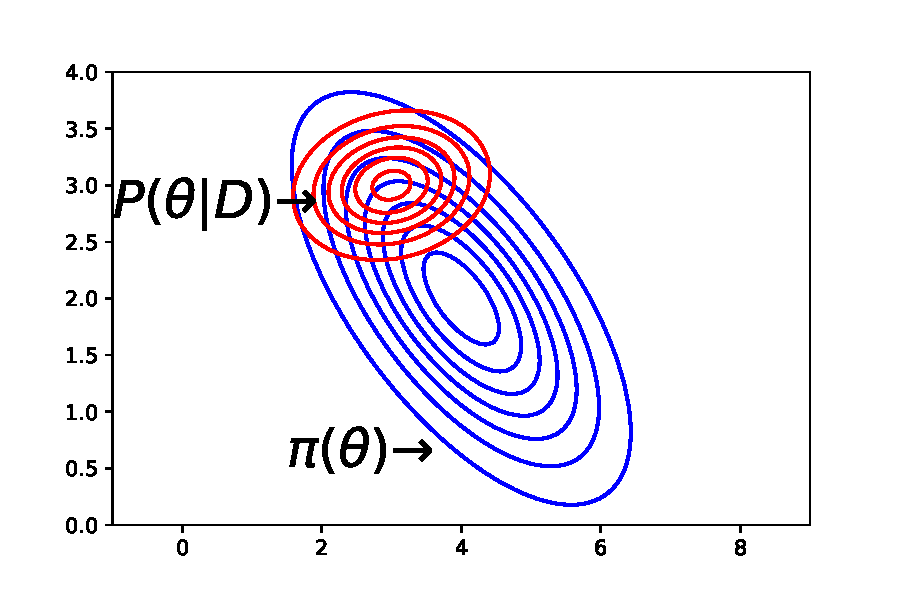
\includegraphics[width=1.1\textwidth]{prior_vs_posterior.pdf}
    %\caption{Caption}
    %\label{fig:my_label}
\end{figure}
\pause
\column{0.5\textwidth}
\begin{figure}[H]
    \centering
    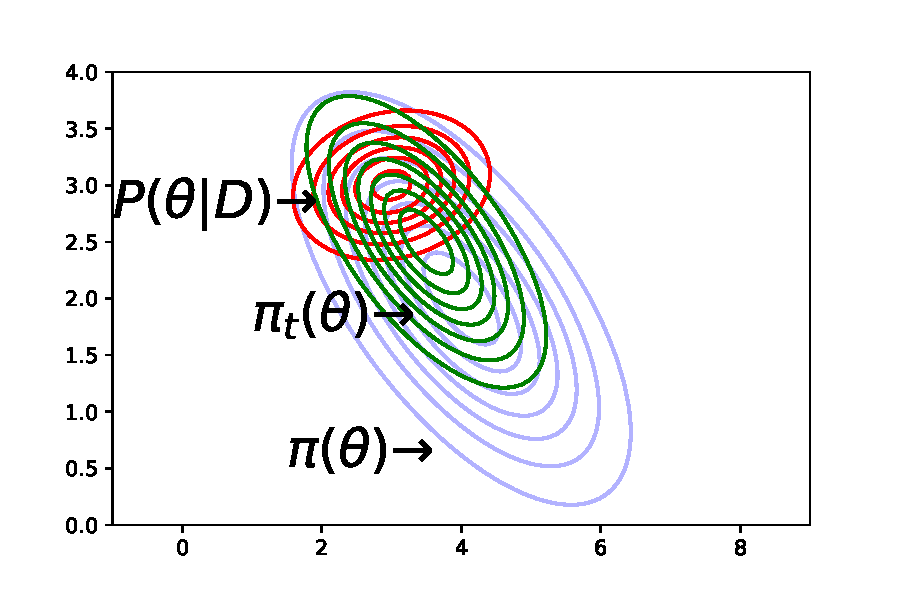
\includegraphics[width=1.1\textwidth]{prior_vs_posterior_with_pi_t.pdf}
    %\caption{Caption}
    %\label{fig:my_label}
\end{figure}
\end{columns}
%\pause
To improve the efficiency we can use what we learned up to time $t$ to build a perturbed prior $\pi_t(\va{\theta})$, which more closely resembles the final posterior
\end{frame}
}

\begin{frame}{Particle-based ABC algorithms}
\begin{itemize}[<+->]
    \item As we noted before ABC methods lend themselves to be parallelized, since each proposal can be sampled and evaluated independently of others being obtained at the same time.
    \item An efficient parallelization scheme (which is also ``intermediate distributions friendly'') is \emph{particle-based sampling}.
    \item We call each sampled parameter a ``particle''. The idea is that we start with a population of particles, then we let them evolve through time so that at each iteration their distribution is closer and closer to the final posterior approximant.
    \item This means that from the particle population at time $t$ we can construct the intermediate distribution $\pi_t$, improve it some way, then resample the population of particles from the new distribution, which is closer to the target.
\end{itemize}
\end{frame}

{\nologo
\begin{frame}{Sequential Importance Sampling (SIS) I}
A possible way to implement the above solution is to build a sequence of distribution $\{\pi_t(\theta)\},  \ t = 1,\dots, T$ using \emph{Sequential Importance Sampling} (SIS). This algorithm works as follows (adapted from \cite{abc_smc}):
\begin{itemize}[<+->]
    \item Let's say we start from a distribution $\pi_1(\theta)$ (e.g. the prior) and we want to get closer and closer to the final distribution $\pi_T$ (e.g. $P_\varepsilon(\theta|y)$, the posterior approximant) in $T$ steps.
    \item In order to get closer and closer to $\pi_T$ the $\pi_t$ distribution should improve the information contained in $\pi_{t-1}$; in the context of SIS/SMC this intuitive idea can be translated e.g. into minimizing the Kullback-Leiber divergence with the target (see e.g. \cite{astroABC}).
    \item Since we're dealing with an evolving population of interactive particles we need to \emph{sample} from each current distribution; this can be achieved by defining $\pi_t$ for any $t$ with \emph{importance sampling}.
\end{itemize}
\end{frame}
}

\begin{frame}{Sequential Importance Sampling (SIS) II}
The idea behind importance sampling is that instead of sampling from $\pi_t$ directly we sample from $\eta_t$, which ideally is a distribution close to $\pi_t$ but easier to sample from; then in order to ``bend'' $\eta_t$ and turn it into $\pi_t$ we rescale probabilities using \emph{importance weights}.


Let us see how this is implemented in practice.
\end{frame}
\begin{frame}{Sequential Importance Sampling (SIS) III}
\begin{itemize}[<+->]
    \item At time $t$ we sample proposals from a population $\{\theta_t^{(i)}\}_{i=1}^N$ of the $i=1, \dots, N$ particles from $\pi_{t-1}$, then perturb them according to $\eta_t$ until we find accepted proposals;
    \item then we evaluate the weights $w_t^{(i)}(\theta_t^{(i)})=\pi_t(\theta_t^{(i)})/\eta_t(\theta_t^{(i)})$ with the accepted proposals i.e. the updated population.
    \item These weights are the discretized version of $\pi_t$, which can be used to sample the to-be-perturbed particle population at the beginning of the next iteration.
\end{itemize}
\pause[\thebeamerpauses]
SIS is a general framework where one is free to choose the distribution sequences $\{\pi_t\}_{t=1}^T$ and $\{\eta_t\}_{t=1}^T$. \emph{ABC Sequential Monte Carlo} (ABC SMC) is the variant where a) $\pi_1$ is the prior, the target $\pi_T$ is the posterior approximant, and each in-between distribution is a more and more ``carved out'' prior, and b) each approximant $\eta_t$ is a \emph{Monte Carlo} estimate of a perturbed version of the previous distribution $\pi_{t-1}$.
\end{frame}

\begin{frame}{ABC Sequential Monte Carlo (ABC SMC) I}
\textit{$\pi_t$ sequence:} In ABC SMC we define:
\begin{equation*}
    \begin{cases}
        \pi_1(\theta) = \pi(\theta) = \text{prior} \\
        \pi_t(\theta) = \pi(\theta) \mathbbm{1}(\rho(y(\theta), y_{\text{obs}}) < \varepsilon_t) \ t = 2, \dots, T-1\\
        \pi_T(\theta) = P_\varepsilon(\theta|y) = \text{posterior approximant}
    \end{cases}
\end{equation*}
In the above $y(\theta)$ is a shorthand notation to mean that $y$ is sampled from the likelihood conditioned on $\theta$, i.e. $y(\theta) \sim \L(y|\theta)$. \pause



\textit{Interpretation:} $\pi_t$ is a ``carved out'' prior. If a specific $\tilde{\theta}$ is incapable of generating a dataset matching the observed one its new probability gets set equal to zero, even if its prior probability is $\pi(\tilde{\theta})\neq 0$. This way we progressively ``remove'' sections of the prior and get closer to the ``smaller'' posterior distribution.
\end{frame}

\begin{frame}{ABC Sequential Monte Carlo (ABC SMC) II}
\textit{$\eta_t$ sequence:} In ABC SMC we define:
\begin{equation*}
    \begin{cases}
        \eta_1(\theta) = \pi_1(\theta) = \pi(\theta)\\
        \eta_t(\theta_t) = \mathbbm{1}(\pi(\theta_t) > 0)\mathbbm{1}(\rho(y(\theta), y_{\text{obs}}) < \varepsilon_t) \int \pi_{t-1}(\theta_{t-1})K_t(\theta_{t-1}, \theta_t)\dd{\theta_{t-1}}
    \end{cases}
\end{equation*}
where we exploited that to get the importance weights we only need to define/compute $\eta_t$ in $\theta_t$, not in an arbitrary $\theta$.
\pause

\textit{Interpretation:} $\eta_t(\theta_t)$ is automatically set to 0 if $\theta_t$ has 0 prior probability and/or is incapable of producing a matching dataset; otherwise it's the perturbed version of the previous distribution $\pi_{t-1}$ via a perturbation kernel $K_t$.
\pause

\textit{$\eta_t(\theta_t)$ evaluation:} notice that $\int \pi_{t-1}(\theta_{t-1})K_t(\theta_{t-1}, \theta_t)\dd{\theta_{t-1}} = \expval{K_t(\theta_{t-1}, \theta_t)}_{\pi_{t-1}}$, which can be approximated as a Monte Carlo average (\emph{Sequential Monte Carlo}).
\end{frame}

\begin{frame}{ABC Sequential Monte Carlo (ABC SMC) III}
Monte Carlo computation of $\eta_t(\theta_t)$:
\begin{equation*}
    \begin{split}
        & \eta_t(\theta_t) = \mathbbm{1}(\pi(\theta_t) > 0)\mathbbm{1}(\rho(y(\theta), y_{\text{obs}}) < \varepsilon_t) \expval{K_t(\theta_{t-1}, \theta_t)}_{\pi_{t-1}} \\
         & \approx \mathbbm{1}(\pi(\theta_t) > 0)\mathbbm{1}(\rho(y(\theta), y_{\text{obs}}) < \varepsilon_t) \cdot \frac{1}{N} \sum_{\theta_{t-1}^{(j)} \sim \pi_{t-1}} K_t(\theta_{t-1}^{(j)}, \theta_t) \\
         & = \mathbbm{1}(\pi(\theta_t) > 0)\mathbbm{1}(\rho(y(\theta), y_{\text{obs}}) < \varepsilon_t) \cdot \frac{1}{N} \sum_{j=1}^N w_{t-1}^{(j)} K_t(\theta_{t-1}^{(j)}, \theta_t)
    \end{split}
\end{equation*}
where $N$ is the n. of particles, and $\{\theta_{t-1}^{(j)}\}_{j=1}^N$ is the population of particles from intermediate distribution $\pi_{t-1}$. 
\end{frame}

\begin{frame}{ABC Sequential Monte Carlo (ABC SMC) IV}
Finally we can write the unnormalized weights for all \emph{accepted} particles $\theta_t$ at any time $t > 1$:
\begin{equation*}
    w_t(\theta_t) = \frac{\pi(\theta_t)}{\eta_t(\theta_t)} = \frac{\pi(\theta_t)}{\sum_{j=1}^N w_{t-1}^{(j)} K_t(\theta_{t-1}^{(j)}, \theta_t)}
\end{equation*}
We now have all elements to write down the final ABC SMC algorithm employed in the \texttt{astroABC} package; adapting again from \cite{abc_smc} we write down the final algorithm.
\end{frame}

\begin{frame}{ABC SMC algorithm I}
\begin{enumerate}[<+->]
    \item Initialize $\varepsilon_1, \dots, \varepsilon_t$.
    \item For each particle sample a proposal $\theta^{**}$ according to the following scheme:
    \begin{itemize}
        \item If $t = 1$ $\theta^{**} \sim \pi(\theta)$;
        \item If $t > 1$ first sample $\theta^*$ from the previous population $\{\theta_{t-1}^{(i)}\}$ \emph{with probabilities given by the weights $w_{t-1}$} and perturb the resulting particle to obtain $\theta^{**}\sim K_t(\theta|\theta^*)$, where $K_t$ is a perturbation kernel.
    \end{itemize}
    \pause[\thebeamerpauses]
    If $\pi(\theta^{**}) = 0$ resample $\theta^{**}$; otherwise simulate a candidate dataset $y^{**}\sim \L(y|\theta^{**})$. If the condition $\rho(y^{**} - y_{\text{obs}}) < \varepsilon_t$ isn't met resample $\theta^{**}$.
\end{enumerate}
\end{frame}
{\nologo
\begin{frame}{ABC SMC algorithm II}
\begin{enumerate}[<+->]
    \setcounter{enumi}{2}
    \item For each particle $i$ set $\theta_t^{(i)}$ equal to their proposal $\theta^{**(i)}$ sampled in the previous step, then for (accepted) particle $\theta_t^{(i)}$ calculate the weight
    \begin{equation*}
        w_t^{(i)} =
        \begin{cases}
            1 \qquad \qquad \qquad \qquad \text{if} \ t = 1\\
            \frac{\pi(\theta_t^{(i)})}{\sum_{j=1}^N w_{t-1}^{(j)} K_t(\theta_{t-1}^{(j)}, \theta_t^{(i)})} \ \text{if} \ t > 1
        \end{cases}
    \end{equation*}
    \item Once all weights have been computed normalize them to 1, then advance to next iteration $t+1$.
\end{enumerate}
\pause[\thebeamerpauses]
Notice how the particles interact: at iteration $t$ each new particle is computed by choosing one from the previous population with \emph{discrete} probabilities $w_{t-1}$ (approximating $\pi_{t-1}$), then perturbed via $K_t$. This means no particles are actually sampled from scratch; we simply let the initial ones evolve so that their collective distribution gets closer to the target density. This allows for trivial parallelization: $\theta_t^{(i)}$ needs $\{\theta_{t-1}^{(j)}\}$ but not the rest of $\{\theta_t^{(i)}\}$ $\implies$ we only need to sync populations at the beginning of $t$ (cfr MCMC).
\end{frame}
}
{\nologo
\begin{frame}{Recap: final \textit{astroABC} algorithm}
\begin{figure}[H]
    \centering
    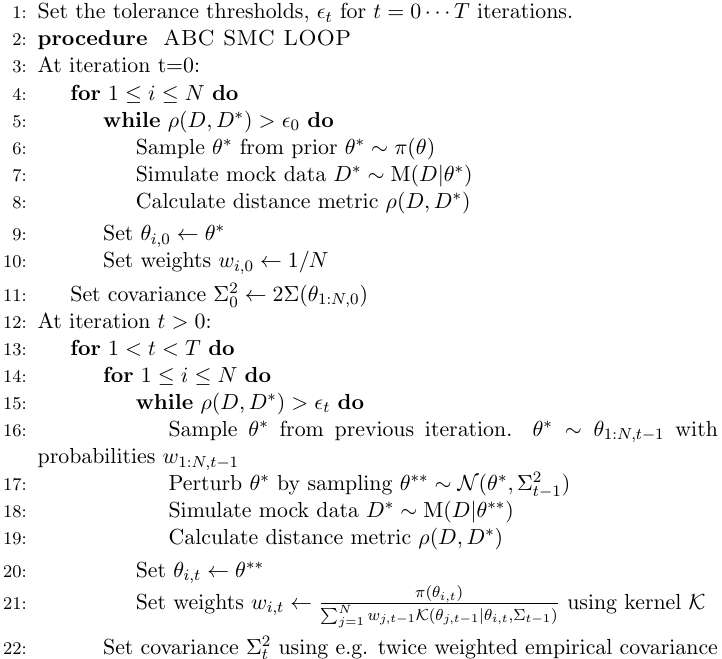
\includegraphics[width=0.7\textwidth, height=0.6\textwidth]{astroabc_algorithm.png}
    %\caption{Main \texttt{astroABC} algorithm.}
    %\label{fig:my_label}
\end{figure}
\end{frame}
}
% ancora non ci siamo, servono altre approssimazioni per rendere efficiente l'algoritmo (anche se tecnicamente adesso funziona): summary statistics (sufficient?), successione di prior dist modificate -> IS con una sola distribuzione intermedia (plot prior + posterior e prior + una sola intermedia + posterior) -> SIS con tante -> SMC se la distribuzione approssimante nel SIS è usata con un approccio Monte Carlo




\section{astroABC}
% varie funzionalità del software (anche la cosa delle covarianze stimate analiticamente o numericamente? boh)
\begin{frame}{astroABC's features I}
\begin{itemize}[<+->]
    \item \textit{Parallelization:} As noted before for fixed $t$ each iteration the loop over particles can be executed in parallel. Each particles is resampled until we find a suitable candidate, and once the full population has been updated we can proceed to $t+1$. This parallel-with-synchronization execution is efficiently implemented in astroABC using \texttt{MPI} for large jobs, and python's \texttt{multiprocessing} for small ones.
    \item \textit{Priors:} astroABC allows the user to assign different prior distributions to each parameter, both standard ones e.g. (gaussians) and custom ones (e.g. implementing the results of previous analyses, which can be done for ex. by supplying previous Markov chains).
    \item \textit{Metric and summary statistics:} astroABC allows the user to define the sufficient statistics and distance metric used in the sampling.
\end{itemize}
\end{frame}

\begin{frame}{astroABC's features II}
\begin{itemize}[<+->]
    \item \textit{ABC SMC:} astroABC allows the user to set at runtime one of a choice of tolerance thresholds, particle covariance estimators and perturbation kernels (more on this later).
    \item \textit{Convenience features:} astroABC allows the user to frequently backup output files and restart files in case a job is canceled due to time restrictions.
\end{itemize}
\end{frame}
\begin{frame}{astroABC's covariance estimators I}
\begin{itemize}[<+->]
    \item In astroABC the distribution covariance is iteratively estimated/refined using the evolving population of particles (instead of computing it once and for all at the start via complex simulations, then fed e.g. in an MCMC-ready likelihood).
    \item The covariance of accepted particles from the previous iteration is used in the SMC adaptive transition kernel $K_t$, which for particle $\theta_t^{(i)}$ is a gaussian kernel with mean $\theta_t^{(i)}$ and covariance equal to this matrix. The user also has the option to use a diagonal covariance matrix (i.e. neglecting correlations between parameters by removing off-diagonal elements) instead of the full matrix.
\end{itemize}
\end{frame}

\begin{frame}{astroABC's covariance estimators II}
To compute the entries in the covariance matrix the following options are available:
\begin{itemize}
    \item twice the empirical covariance amongst the particles;
    \item covariances which result in a kernel which minimizes the Kullback-Leibler divergence between the target distribution and the distribution of the perturbed particles;
    \item local covariance estimate using scikit-learn’s \texttt{KDTree} method for nearest neighbours;
    \item twice the weighted particle covariance matrix;
    \item a shrinkage covariance metric with the Ledoit-Wolf estimator.
\end{itemize}
Nontrivial options in the above list are motivated/discussed in the astroABC paper's references.
\end{frame}

{\nologo
\begin{frame}{astroABC's tolerance level scheduler I}
\begin{itemize}[<+->]
    \item As we know if $\varepsilon$ is too large we recover the prior $\implies$ we learn nothing, whereas if $\varepsilon$ is too small too many samples are rejected $\implies$ the algorithm is so picky it becomes too inefficient. 
    \item Achieving a balance between these two cases can be hard; instead of finding a single good value for $\varepsilon$ we can define a decreasing sequence $\{\varepsilon_t\}$.
    \item At the beginning we haven't yet learned much, so in order to get closer to the posterior it makes sense to have a larger tolerance i.e. to accept even parameters that don't represent the observed data with high accuracy.
    \item Similarly as the algorithm progresses we can afford lower efficiency because we already have an approximation of the posterior, and what we need is to improve it with high accuracy estimates. For this reason the tolerance level decreases over time, so that later on the parameters are sampling a high probability region of the posterior distribution.
\end{itemize}
\end{frame}
}

\begin{frame}{astroABC's tolerance level scheduler II}
\begin{itemize}[<+->]
    \item Within astroABC users can select a linearly decreasing, log decreasing, exponentially decreasing, constant or iteratively adaptive tolerance threshold. 
    \item For the iteratively adaptive option the user specifies a certain quantile e.g. 75th, of the metric distance from the previous iteration. As such this decreasing tolerance depends on the particle positions in the previous iteration.
    \item All tolerances require an input maximum and minimum value and the selected tolerance type is then implemented from a maximum value until either the minimum value is reached or the particles have reached the maximum number of iterations requested.
\end{itemize}    
\end{frame}

\section{MCMC vs ABC: example supernovae analysis}
% grafici del paper, skew normal che puoi graficare con matplotlib al volo
\begin{frame}{astroABC paper's example}
Citing directly from \cite{astroABC}: ``In this section we present a simple example of parameter inference, with a simulated supernovae dataset, using both a standard MCMC sampler and astroABC. \emph{This example represents a nontrivial case which has been specifically chosen to highlight potential biases in the MCMC approach which can be avoided using ABC.} Note this is not meant to show the best constraints we can get from ABC versus MCMC using supernova data. \emph{The toy example is meant to breakdown key elements and assumptions about the two methods with a simple physical example} and is intended as a teaching exercise.''


Similar situation as in the BHM SN Ia paper, but where we purposely ``cheat'' to make the BHM rigorous approach fail in a way that is automatically prevented by using ABC.
\end{frame}

\begin{frame}{Problem setup}
\begin{itemize}[<+->]
    \item In this example a mock dataset of 400 supernovae in the $0.5 < z < 1.0$ redshift range is sampled using the following ``true'' values:
    \begin{itemize}
        \item Matter density of the universe today: $\Omega_m = 0.3$
        \item Dark energy density of the universe today: $\Omega_\Lambda = 0.7$
        \item Present value of the dark energy equation of state: $w_0 = -1.0$
    \end{itemize}
    \item At every redshift we add \emph{non gaussian noise} by adding random variates from a skewed normal distribution with fixed parameters: location $= -0.1$, scale $= 0.3$, skew $= 5.0$; this is the crucial point, more on this in the next slide
    \item During sampling we assume a flat universe and no prior information from other probes; we only assume wide gaussian priors on both parameters:
    \begin{itemize}
        \item $\pi(\Omega_m) = \N(0.3, 0.5)$
        \item $\pi(w_0) = \N(-1, 0.5)$
    \end{itemize}
\end{itemize}
\end{frame}

{\nologo
\begin{frame}{Non-Gaussian noise I}
\begin{figure}[H]
    \centering
    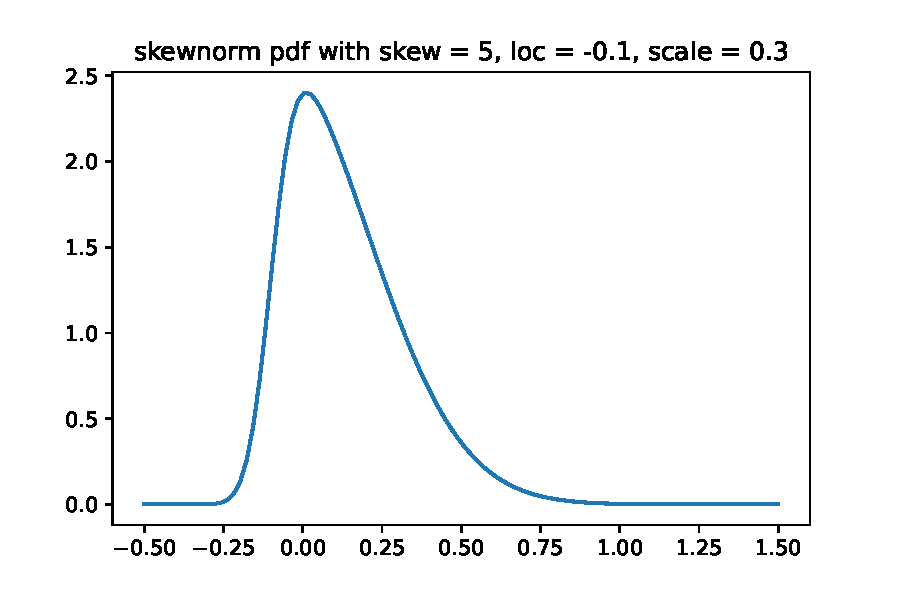
\includegraphics[width=0.6\textwidth]{skewnorm.pdf}
    %\caption{Caption}
    %\label{fig:my_label}
\end{figure}
\begin{itemize}%[<+->]
    \item Adding this non-Gaussian random noise means that the final dataset has a non-Gaussian distribution at every redshift. In realistic datasets there may be several systematics which will have a similar effect e.g zero-point offset systematics in supernova studies.
\end{itemize}
\end{frame}
}

\begin{frame}{Non-Gaussian noise II}
\begin{itemize}[<+->]
    \item We assume that an analytic expression for the distribution of the final dataset is not available to us, but that e.g. non gaussian systematics can be accurately forward modeled using a simulation.
    \item For this reason \emph{in the context of this example} sticking to a Gaussian likelihood is inaccurate yet basically unavoidable within an MCMC approach; if instead we use ABC we may use the same physical model without also needing the full likelihood (more on this later).
\end{itemize}
\pause[\thebeamerpauses]
For now let us setup each model and see the results.
\end{frame}
{\nologo
\begin{frame}{MCMC setup}
In this toy example we assume a simple gaussian likelihood without realistic complications (like e.g. nonconstant absolute magnitude, which aren't present in the simple mock dataset):
\begin{equation*}
    \L(\mu_{\text{data}}|\mu_{\text{model}}(z, \Omega_m, w_0))\propto \exp(-\sum_i \tonde{\frac{\mu_{\text{data}}^i - \mu_{\text{model}}(z^i, \Omega_m, w_0)}{2\sigma^i}}^2 )
\end{equation*}
where $\mu_{\text{data}}^i$ is the distance modulus for an individual supernova in the data, with associated error $\sigma^i$, and where (flat universe assumption)
\begin{equation*}
    \mu_{\text{model}}(z^i, \Omega_m, w_0)\propto 5\log_{10}\frac{c(1+z)}{h_0}\int_0^{z^i}\dd{z'}\frac{1}{E(z')}
\end{equation*}
\begin{equation*}
    E(z) = \sqrt{\Omega_m (1+z)^3 + (1-\Omega_m)\exp(3\int_0^z\dd{\ln(1+z')}(1+w(z')))}
\end{equation*}
\end{frame}
}

\begin{frame}{MCMC results I}
With this MCMC and 28 chains with $10^5$ points each the results are the following:
\begin{figure}[H]
    \centering
    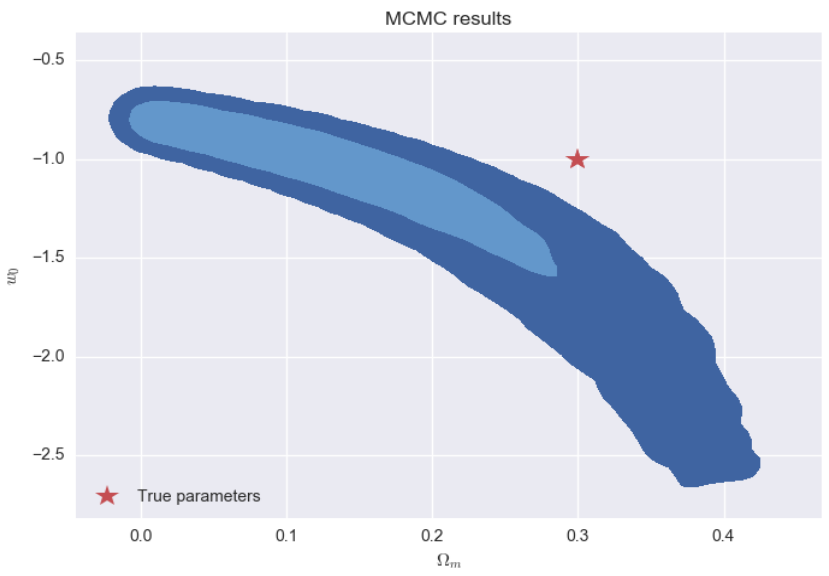
\includegraphics[width=0.6\textwidth]{astroabc_mcmc_results.png}
    \caption{$P_{\text{MCMC}}(\Omega_m, w_0|D)$ with $1\sigma$ and $2\sigma$ contours shown.}
    %\label{fig:my_label}
\end{figure}
\end{frame}

\begin{frame}{MCMC results II}
\begin{itemize}[<+->]
    \item The true parameters are clearly outside of the $2\sigma$ credibility region. This is also confirmed by the $1\sigma$ marginalized best fit values: $\Omega_m = 0.17\pm 0.11$, $w_0 = -1.26\pm 0.55$. Even though the ``true'' value $-1.0$ for $w_0$ is within its $1\sigma$ interval $\Omega_m = 0.3$ clearly isn't, as can be seen in the previous plot.
    \item \emph{It is clear that the simple Gaussian Likelihood assumption in this case (which neglects the effects of systematics) yields biased cosmological constraints.}
    \item We can do better with ABC in this specific instance.
\end{itemize}
\end{frame}

{\nologo
\begin{frame}{ABC setup I}
\begin{itemize}[<+->]
    \item In this toy example we assume that our noisy data can be simulated accurately and easily, but that an analytical expression for the likelihood is not available to us.
    \item Using a forward model simulation we can account for non-Gaussian uncertainties in the data without explicitly knowing the likelihood. In particular we assume our simulation is able to draw gaussian random variates from the same $\mu_{\text{model}}(z^i, \Omega_m, w_0) = \dots$ model, \emph{to which we add non-Gaussian noise from a skew normal distribution} (i.e. the systematics).
    \item \emph{Remark:} the use of exactly the same model here in the two methods is to highlight the distinction between choice of \emph{model}, and choice of \emph{Likelihood} in inference techniques. \emph{Even though the physical model can be the same in both, an incorrect Likelihood assumption can bias results.}
\end{itemize}
\end{frame}
}

\begin{frame}{ABC setup II}
\begin{itemize}[<+->]
    \item Also notice that with ABC it is also possible to parametrize the source of non-Gaussian noise in the simulation and fit for e.g. the hyperparameters of the skew normal distribution, too.
    \item Using ABC at every iteration we simulate a set of supernovae at every point in a two dimensional parameter space $\{(\Omega_m, w_0)\}$; this simulated output is then compared with the dataset using a weighted Euclidean metric and an iteratively adaptive threshold.
    \item In the paper the authors use 100 particles and run until the error on the $1\sigma$ contour is $\sim 5\%$; this choice for the number of particles is based on trial and error runs to determine an optimal way to sample a multi dimensional parameter space efficiently.
\end{itemize}
\pause[\thebeamerpauses]
First let us plot the progress of the ABC particles as a function of time, compared to the true values (red star).
\end{frame}

{\nologo
\begin{frame}{ABC results I}
\begin{figure}[H]
    \centering
    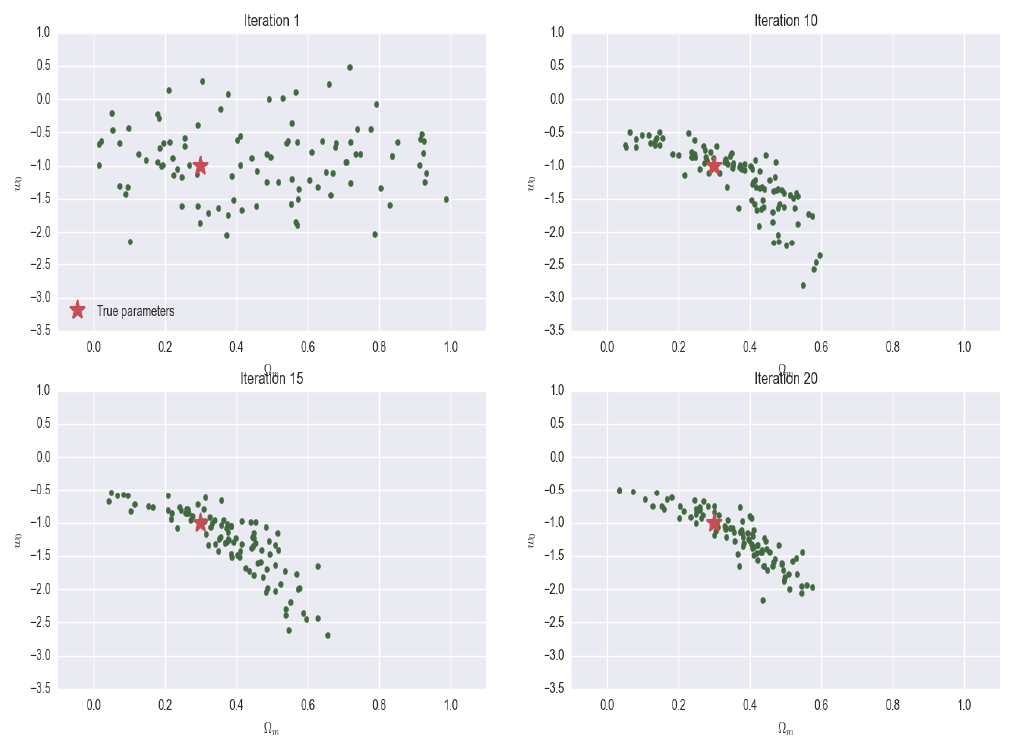
\includegraphics[width=0.7\textwidth]{astroabc_abc_results_1.png}
    %\caption{Caption}
    %\label{fig:my_label}
\end{figure}
It is clear that at $t=1$ the particles are well dispersed throughout the prior range. As the tolerance
threshold level decreases the particles converge towards the ``true'' values, distributing like the posterior.
\end{frame}
}

\begin{frame}{ABC results II}
\begin{figure}[H]
    \centering
    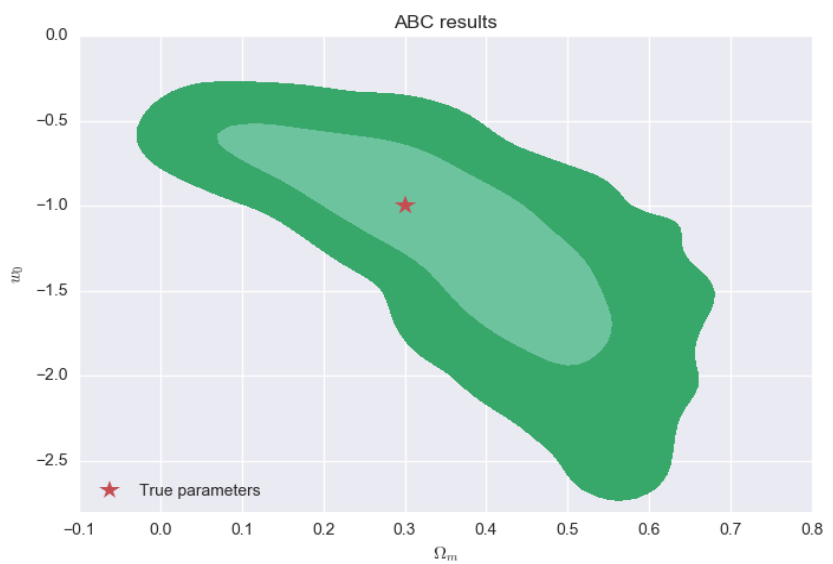
\includegraphics[width=0.6\textwidth]{astroabc_abc_results_2.png}
    \caption{$P_{\text{ABC}}(\Omega_m, w_0|D)$ with $1\sigma$ and $2\sigma$ contours shown.}
    %\label{fig:my_label}
\end{figure}
This time the posterior is clearly unbiased, and accurately centered on the ``true'' values.
\end{frame}

\begin{frame}{ABC results III}
\begin{itemize}[<+->]
    \item The $1\sigma$ marginalized best fit values are $\Omega_m = 0.36\pm 0.12$, $w_0 = -1.22\pm 0.4$ inside which the true values comfortably sit. 
    \item It's evident that with a forward simulation model one can naturally incorporate systematic effects at every point in parameter space, while avoiding the explicit calculation of the Likelihood and any parameter bias seen in the MCMC method.
\end{itemize}
\end{frame}


\section{Conclusions}
% serve davvero? Probabilmente basta una conclusione riassuntiva
{\nologo
\begin{frame}{Conclusions}
From the astroABC paper \cite{astroABC}: ``We have described astroABC [\dots] [its] sampler can be used in parameter inference by simulating observations from posterior distributions when likelihoods are difficult or impossible to compute. Problems such as this arise frequently in cosmological applications, where [\dots] often [\dots] a physical model for the data can be simulated rapidly, and [\dots] [with] systematic uncertainties, but is sufficiently complicated that explicit formulae for the Likelihood are not known. The demand for alternative sampling methods in astronomy is increasing given the large correlated datasets we expect to analyze from future surveys. Current methods increasingly rely on simulations for error estimation and ABC sampling is a natural extension of this approach with the advantage that the Likelihood is not explicitly calculated. astroABC was designed to be [\dots] user friendly [\dots] while also accommodating the computational demands of simulating future datasets [\dots] with its facility for massive parallelization using MPI [\dots] and innovative factors such as a varied choice of covariance and kernel estimation, tolerance levels and priors.''
\end{frame}
}


{\nologo
\begin{frame}[allowframebreaks]{Bibliography}
%\fontsize{6pt}{7.2}\selectfont
\nocite{*}
\printbibliography%[heading=bibintoc]    %tolgo quella opzione per non fare spuntare la bibliografia nella toc=table of contents
\end{frame}
}



\end{document}
